\documentclass[12pt]{scrartcl}
\title{Take home exam II}
\nonstopmode
%\usepackage[utf-8]{inputenc}
\usepackage{array}
\usepackage{tabularx}
\usepackage{graphicx} % Required for including pictures
\usepackage[figurename=Figure]{caption}
\usepackage{float}    % For tables and other floats
\usepackage{verbatim} % For comments and other
\usepackage{amsmath}  % For math
\usepackage{amssymb}  % For more math
\usepackage{fullpage} % Set margins and place page numbers at bottom center
\usepackage{paralist} % paragraph spacing
\usepackage{listings} % For source code
\usepackage{subfig}   % For subfigures
%\usepackage{physics}  % for simplified dv, and 
\usepackage{enumitem} % useful for itemization
\usepackage{siunitx}  % standardization of si units
\usepackage[spanish,es-tabla]{babel}
\usepackage[utf8]{inputenc}
\usepackage{multicol}
\usepackage{multirow} % para las tablas
\usepackage{enumitem}
\usepackage{xcolor}
\usepackage{hyperref}
\usepackage{tikz}
\usepackage{color, colortbl}
\usepackage[margin=0.8in]{geometry} % for PAPER & MARGIN
\usepackage[many]{tcolorbox}    	% for COLORED BOXES (tikz and xcolor included)
\usepackage{setspace}               % for LINE SPACING
\usepackage{multicol}               % for MULTICOLUMNS
\usepackage{graphicx}
\usepackage{subfigure}
\usepackage{listings}
\usepackage{pythontex} 
\usepackage[utf8]{inputenc}
\usepackage[T1]{fontenc}
\setlength{\parindent}{0pt}
\usepackage{tcolorbox}
\tcbuselibrary{minted,breakable,xparse,skins}

\definecolor{bg}{gray}{0.95}
\DeclareTCBListing{mintedbox}{O{}m!O{}}{%
  breakable=true,
  listing engine=minted,
  listing only,
  minted language=#2,
  minted style=default,
  minted options={%
    linenos,
    gobble=0,
    breaklines=true,
    breakafter=,,
    fontsize=\small,
    numbersep=8pt,
    #1},
  boxsep=0pt,
  left skip=0pt,
  right skip=0pt,
  left=25pt,
  right=0pt,
  top=3pt,
  bottom=3pt,
  arc=5pt,
  leftrule=0pt,
  rightrule=0pt,
  bottomrule=2pt,
  toprule=2pt,
  colback=bg,
  colframe=orange!70,
  enhanced,
  overlay={%
    \begin{tcbclipinterior}
    \fill[orange!20!white] (frame.south west) rectangle ([xshift=20pt]frame.north west);
    \end{tcbclipinterior}},
  #3}

%\setlength\columnsep{0.25in} % setting length of column separator
\definecolor{main}{HTML}{5989cf}    % setting main color to be used
\definecolor{sub}{HTML}{cde4ff}     % setting sub color to be used

\definecolor{commentgreen}{RGB}{2,112,10}
\definecolor{highlightblue}{RGB}{31,119,220}
\definecolor{eminence}{RGB}{108,48,130}
\definecolor{weborange}{RGB}{255,129,0}
\definecolor{frenchplum}{RGB}{129,20,83}
\definecolor{darkpink}{RGB}{229,4,101}
\definecolor{gray}{gray}{0.9}


\tcbset{
    sharp corners,
    colback = white,
    before skip = 0.2cm,    % add extra space before the box
    after skip = 0.5cm      % add extra space after the box
}                           % setting global options for tcolorbox

\newtcolorbox{boxF}{
    colback = sub,
    enhanced,
    boxrule = 1.5pt, 
    colframe = white, % making the base for dash line
    borderline = {1.5pt}{0pt}{main, dashed} % add "dashed" for dashed line
}

\newtcolorbox{boxK}{
    sharpish corners, % better drop shadow
    boxrule = 0pt,
    toprule = 2pt, % top rule weight
    enhanced,
    fuzzy shadow = {0pt}{-2pt}{-0.5pt}{0.5pt}{black!35} % {xshift}{yshift}{offset}{step}{options} 
}


%%% Colours used in field vectors and propagation direction
\definecolor{mycolor}{rgb}{1,0.2,0.3}
\definecolor{brightgreen}{rgb}{0.4, 1.0, 0.0}
\definecolor{britishracinggreen}{rgb}{0.0, 0.26, 0.15}
\definecolor{cadmiumgreen}{rgb}{0.0, 0.42, 0.24}
\definecolor{ceruleanblue}{rgb}{0.16, 0.32, 0.75}
\definecolor{darkelectricblue}{rgb}{0.33, 0.41, 0.47}
\definecolor{darkpowderblue}{rgb}{0.0, 0.2, 0.6}
\definecolor{darktangerine}{rgb}{1.0, 0.66, 0.07}
\definecolor{emerald}{rgb}{0.31, 0.78, 0.47}
\definecolor{palatinatepurple}{rgb}{0.41, 0.16, 0.38}
\definecolor{pastelviolet}{rgb}{0.8, 0.6, 0.79}


\hypersetup{%
    colorlinks=True,
    urlcolor=darkpowderblue,
    citecolor=darkpowderblue,
    linkcolor=darkpowderblue
    }


\begin{document}

\begin{center}
	\hrule
	\vspace{.4cm}
	{\textbf { \large \textbf{Práctica 1} \\ APPIV \\ \vspace{1em} \small \textit{Clasificación de imágenes. Arquitecturas CNN. Transfer Learning.}} \\ \vspace{0.5em}\today}
\end{center}

\begin{center}
{ \vspace{0.5em} Gloria del Valle Cano \hspace{\fill}   \\}
{ gloria.valle@estudiante.uam.es \hspace{\fill} \\ \vspace{1.5em}}
	\hrule
\end{center}



%%%%%%%%%%%%%%%%%%%%%%%%%%%%%%%%%%%%%%%%%%%%%%%%%%%%%%%%%%%%%%%%%%%%%%%%%%%%%%%%%%%%%%%%%%%%%%%%%%%%%%%%%%%%%%%
\section{Simple CNN}

\begin{itemize}
    \item Tamaños de los conjuntos de entrenamiento y validación descargados del dataset MNIST.
    \begin{table}[H]
        \centering
        \begin{tabular}{l c c c c}
            \multicolumn{1}{c}{}                & \cellcolor[HTML]{E3E7EC}Alto & \cellcolor[HTML]{E3E7EC}Ancho & \cellcolor[HTML]{E3E7EC}Nº de canales & \cellcolor[HTML]{E3E7EC}Nº de muestras \\ \hline
            \cellcolor[HTML]{E3E7EC}Entrenamiento & 28                                        & 28                                         & 1                                               & 60000                                  \\
            \cellcolor[HTML]{E3E7EC}Validación    & 28                                        & 28                                         & 1                                               & 10000                                  \\ 
        \end{tabular}
        \caption{Resumen del tamaño de los conjuntos de \emph{train} y \emph{valid}.}
        \label{table:res1}
    \end{table}
    \item Número de parámetros del modelo Simple CNN.
    \begin{table}[H]
        \centering
        \begin{tabular}{l c}
            \multicolumn{1}{c}{}             & \cellcolor[HTML]{E3E7EC}Número de parámetros del modelo Simple CNN \\ \hline
            \cellcolor[HTML]{E3E7EC}Simple CNN & 813802                                                             \\
        \end{tabular}
        \caption{Resumen del número de parámetros del modelo.}
        \label{table:res1}
    \end{table}
    \item Incluya las curvas de entrenamiento y validación para 10 épocas. Indique también la mejor precisión obtenida, y en qué época se logra este resultado. Comentar las conclusiones sobre la evolución de la loss de entrenamiento y validación, con respecto a posibles problemas de sesgo (high-bias) o sobreajuste (overfitting). Indique si considera que continuar con más épocas de entrenamiento mejoraría el rendimiento del modelo.
    \begin{figure}[H]
        \centering
        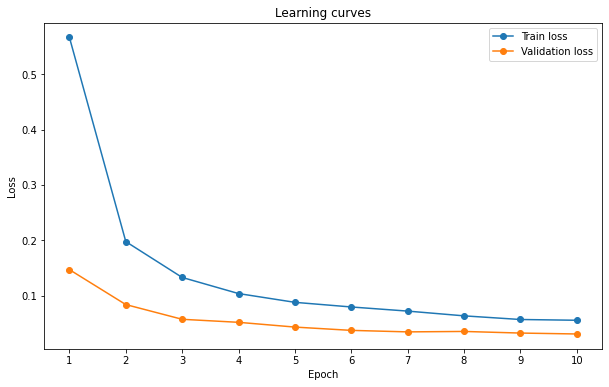
\includegraphics[scale=0.48]{curvas1.png}
        \caption{Curvas de entrenamiento y validación para el modelo Simple CNN. Épocas 1-10.}
        \label{fig:curvas1}
    \end{figure}
    
    Como podemos ver en la Figura \ref{fig:curvas1}, la función de pérdida va decreciendo mucho más en el conjunto de validación que en el conjunto de entrenamiento, por lo que vemos que no hay \emph{overfitting}.
    Es posible que este efecto se deba a la inclusión del \emph{Dropout} en entrenamiento, ya que esto regulariza por la capacidad de ignorar determinadas neuronas durante el entrenamiento. Tampoco se observan 
    problemas de \emph{high-bias}, ya que la pérdida siempre decrece, por lo que podemos ver que el modelo está aprendiendo.

    \begin{table}[H]
        \centering
        \begin{tabular}{l c l}
        \multicolumn{1}{c}{}             & \cellcolor[HTML]{E3E7EC}Mejor precisión (validación) & \cellcolor[HTML]{E3E7EC} Época con mejor precisión \\ \hline
        \cellcolor[HTML]{E3E7EC}Simple CNN & 98.94\%                                              & \multicolumn{1}{c}{10}   \\ 
        \end{tabular}
        \caption{Mejor precisión con su correspondiente época, obtenida por el modelo.}
        \label{table:resultsprec}
        \end{table}

    La mejor precisión obtenida se alcanza en la última época (ver Tabla \ref{table:resultsprec}), siendo ésta bastante alta. Vista la progresión de los resultados en cada época (ver primer notebook) y las curvas de aprendizaje,
    es muy posible que el modelo siguiera aprendiendo un poco más. Comprobamos esta suposición más tarde, con 10 épocas más. Adjuntamos los resultados
    en la Figura \ref{fig:curvas12}.
    \begin{figure}[H]
        \centering
        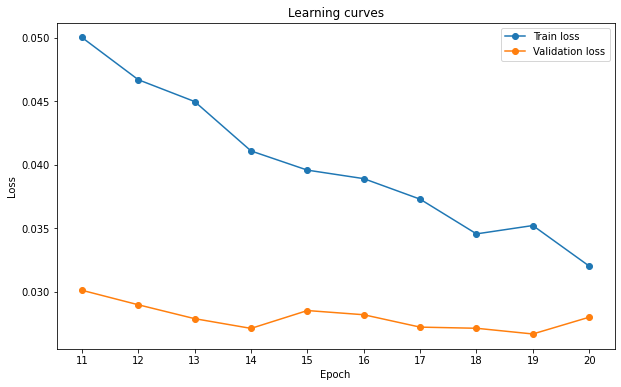
\includegraphics[scale=0.48]{curvas12.png}
        \caption{Curvas de entrenamiento y validación para el modelo Simple CNN. Épocas 11-20.}
        \label{fig:curvas12}
    \end{figure}
    Viendo los resultados en el notebook, conseguimos aumentar la precisión a $99.10\%$ en la época $19$. Observando el comportamiento de la curva y de los resultados, es muy posible que el aprendizaje se hubiera estancado en ese punto.

    \item Incluir la matriz de confusión obtenida. Dada esta matriz de confusión, informe de los 2 casos de confusión entre clases que ocurren con más frecuencia.
    \begin{figure}[H]
        \centering
        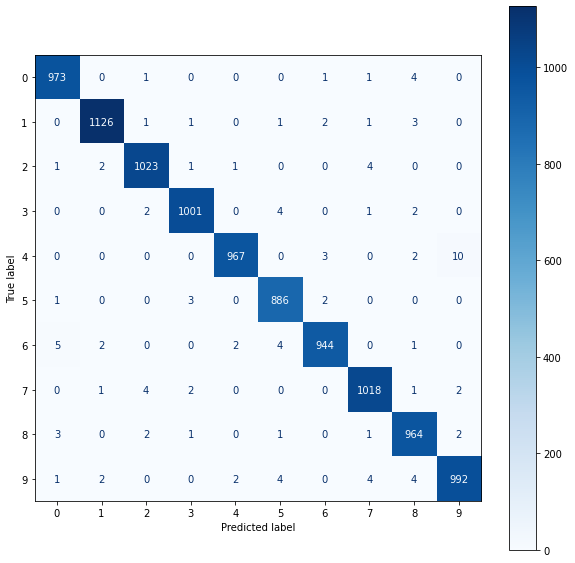
\includegraphics[scale=0.58]{confmatrx1.png}
        \caption{Matriz de confusión de Simple CNN (10 épocas).}
        \label{fig:confmatrx1}
    \end{figure}
    Viendo los resultados, observamos que obtenemos un total de 106 errores de un total de 10000 predicciones. Los errores más comunes se encuentran en el dígito $6$ (tiene muchas confusiones con el $0$, el $5$, etc.), el $4$ (se suele confundir con el $9$), el $5$, incluso el $8$. Podemos ver mejor algunas de estas confusiones en la Figura \ref{fig:errores1}.
    \begin{figure}[H]
        \centering
        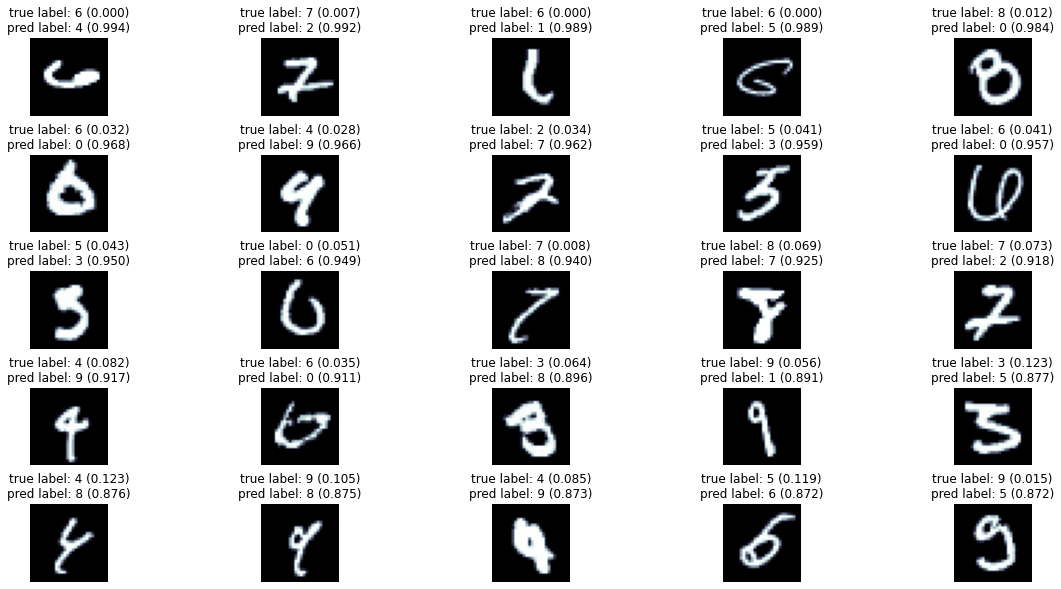
\includegraphics[scale=0.42]{mosterror1.png}
        \caption{Ejemplos de dígitos con más errores en la clasificación.}
        \label{fig:errores1}
    \end{figure}
    
    \item Comente las diferencias entre el gráfico t-SNE de la representación de las capas final e intermedia de la CNN, aplicado a las imágenes del conjunto de validación. Para ello, considere la proximidad y la dispersión entre los clústeres en ambas representaciones, y su relación con la capacidad de realizar una correcta clasificación de las muestras.
    \begin{figure}[H]
        \centering
        \subfigure[Representación intermedia]{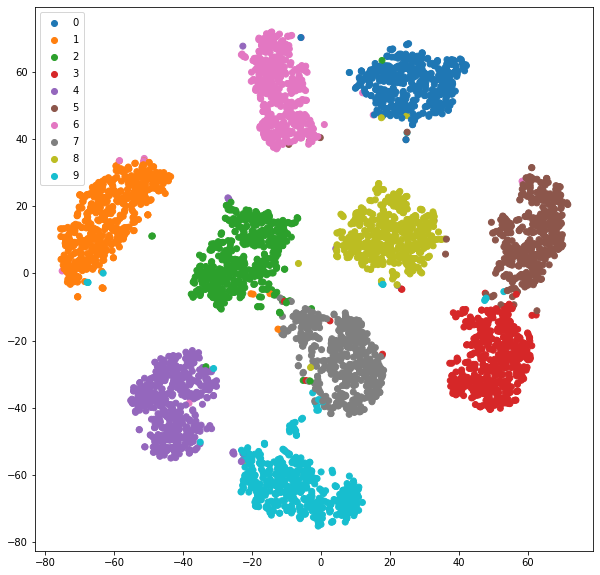
\includegraphics[width=0.4\textwidth]{t-sne2.png}}                
        \subfigure[Representación final]{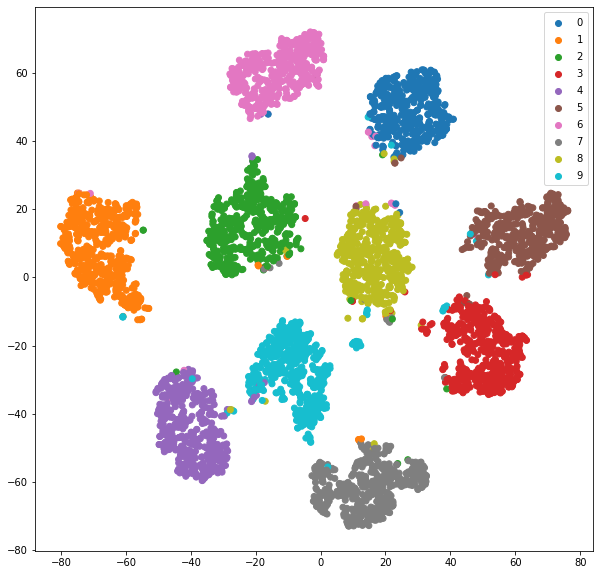
\includegraphics[width=0.4\textwidth]{t-sne1.png}}
        \caption{Representaciones t-SNE.}
        \label{fig:tsne1}
    \end{figure}
    
    Como vemos en la Figura \ref{fig:tsne1} obtenemos 10 clases completamente diferenciadas por clusters, por lo que parece que la red clasifica con éxito los dígitos aun con sus pocos fallos.
    Sí que es verdad que en la representación intermedia observamos que hay un poco de solapamiento en las clases $5$ y $3$ y en el $2$ y el $7$, si bien en la representación final vemos que 
    este efecto se ha mitigado.
    
    \item Dadas las diferencias entre la representación t-SNE de ambas capas, y dada la arquitectura de la red implementada, identifique en qué capa de la red se extraen las características, y proponga una forma de reducir la complejidad de la red, con una penalización baja en la precisión de la clasificación.
    
    Observando la arquitectura de esta red vemos que las características se extraen antes de la primera capa \emph{Linear}. Una manera de reducir la complejidad de la red sería eliminar la última capa lineal ya que parece que la diferencia entre ambas representaciones no es vital y el error no sería muy alto.
    
    \end{itemize}
    
\section{AlexNet}
\begin{itemize}
    \item Incluya el código que ha utilizado para definir la clase \texttt{AlexNet}.
    
    
    \begin{mintedbox}{python}
    class AlexNet(nn.Module):
            def __init__(self, output_dim):
                super().__init__()
                
                self.features = nn.Sequential(
                    # First convolutional layer. Use 5x5 kernel instead of 11x11
                    nn.Conv2d(3, 48, 5, 2, 2), #in_channels, out_channels, kernel_size, stride, padding
                    nn.MaxPool2d(2), #kernel_size
                    nn.ReLU(inplace = True),
                    # Complete the following four conv layers of the AlexNet model. 
                    # Subsampling is only performed by 2x2 max pooling layers (not with stride in the 
                    # convolutional layers)
                    # Pay special attention to the number of input and output channels of each layer
                    nn.Conv2d(48, 128, 5, 1, 2),
                    nn.MaxPool2d(2),
                    nn.ReLU(inplace=True),

                    nn.Conv2d(128, 192, 3, 1, 1),
                    nn.ReLU(inplace=True),
                    nn.Conv2d(192, 192, 3, 1, 1),
                    nn.ReLU(inplace=True),

                    nn.Conv2d(192, 128, 3, 1, 1),
                    nn.MaxPool2d(2),
                    nn.ReLU(inplace=True)
                )
                
                self.classifier = nn.Sequential(
                    # First linear layer
                    nn.Dropout(0.5),
                    nn.Linear(128 * 2 * 2, 2048), # final conv layer resolution 2x2
                    nn.ReLU(inplace = True),
                    # second linear layer
                    nn.Dropout(0.5),
                    nn.Linear(2048, 2048),
                    nn.ReLU(inplace=True),
                    
                    # Last Linear layer. No ReLU
                    nn.Linear(2048, output_dim),
                )

            def forward(self, x):
                x = self.features(x)
                interm_features = x.view(x.shape[0], -1)
                x = self.classifier(interm_features)
                return x, interm_features
\end{mintedbox}

\item Número de parámetros del modelo \texttt{AlexNet}.

Con \texttt{summary} de \texttt{torchsummary} podemos ver este resultado.
\begin{table}[H]
\centering
\begin{tabular}{l c}
\multicolumn{1}{c}{}          & \cellcolor[HTML]{E3E7EC}Nº parámetros entrenables \\ \hline
\cellcolor[HTML]{E3E7EC}AlexNet & 6 199 498                                         \\
\end{tabular}
\caption{Resumen del número de parámetros entrenables del modelo.}
\label{table:alexnetparams}
\end{table}
\item Incluya las curvas de entrenamiento y validación para 15 épocas. Indique también la mejor precisión obtenida, y en qué época se logra este resultado. Comentar las conclusiones sobre la evolución de la loss de entrenamiento y validación, y comentar lo que posiblemente está sucediendo después de la época 10. Indique si considera que continuar con más épocas de entrenamiento mejoraría el rendimiento del modelo.

\begin{figure}[H]
        \centering
        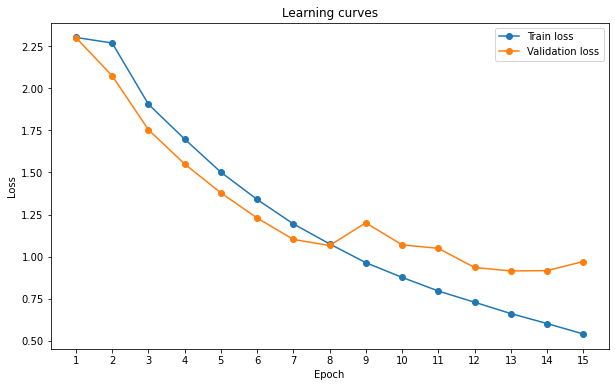
\includegraphics[scale=0.48]{curvasalex1.png}
        \caption{Curvas de entrenamiento y validación para el modelo AlexNet. Épocas 1-15.}
        \label{fig:curvasalex1}
    \end{figure}
    
Las curvas de entrenamiento y validación se pueden ver en la Figura \ref{fig:curvasalex1}. Vemos que esta vez el dataset es mucho más difícil de aprender y utilizando un modelo como AlexNet obtenemos la precisión que se observa en la Tabla \ref{table:resultsprecalex}. También observamos que la pérdida va descenciendo como se espera, si bien a partir de la época 8 la loss de validación empieza a aumentar, por lo que el modelo está empezando a sobreajustar. Vemos que entre 8 y, tal vez, 12 épocas sería suficiente y que muchas más no sería beneficioso para el rendimiento del modelo.
    
\begin{table}[H]
        \centering
        \begin{tabular}{l c l}
        \multicolumn{1}{c}{}             & \cellcolor[HTML]{E3E7EC}Mejor precisión (validación) & \cellcolor[HTML]{E3E7EC} Época con mejor precisión \\ \hline
        \cellcolor[HTML]{E3E7EC} AlexNet & 71.22\%                                              & \multicolumn{1}{c}{14}   \\ 
        \end{tabular}
        \caption{Mejor precisión con su correspondiente época, obtenida por el modelo.}
        \label{table:resultsprecalex}
        \end{table}
\item Incluir la matriz de confusión. Comentar los resultados obtenidos atendiendo a las características de las imágenes de cada clase.

\begin{figure}[H]
        \centering
        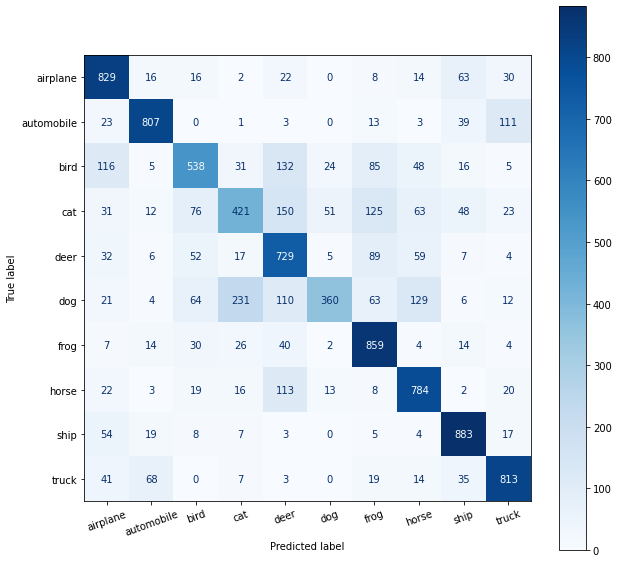
\includegraphics[scale=0.58]{confalex1.png}
        \caption{Matriz de confusión de AlexNet (15 épocas).}
        \label{fig:confmatrx2}
\end{figure}
Según vemos en la Figura \ref{fig:confmatrx2}, las clases que obtienen más errores son las de \emph{dog}, \emph{cat} (se confunden entre sí bastante) y \emph{horse}, que se suele confundir con \emph{deer}. Esto puede tener sentido porque pueden ser parecidos entre sí por tamaño, color e incluso por los fondos, ya que los últimos se encuentran más en la naturaleza, mientras que los gatos y los perros son domésticos. También observamos confusiones entre \emph{automobile} y \emph{truck}, lo que parece igual de lógico. Podemos ver ejemplos de esto en la Figura \ref{fig:mosterror2}.

\begin{figure}[H]
        \centering
        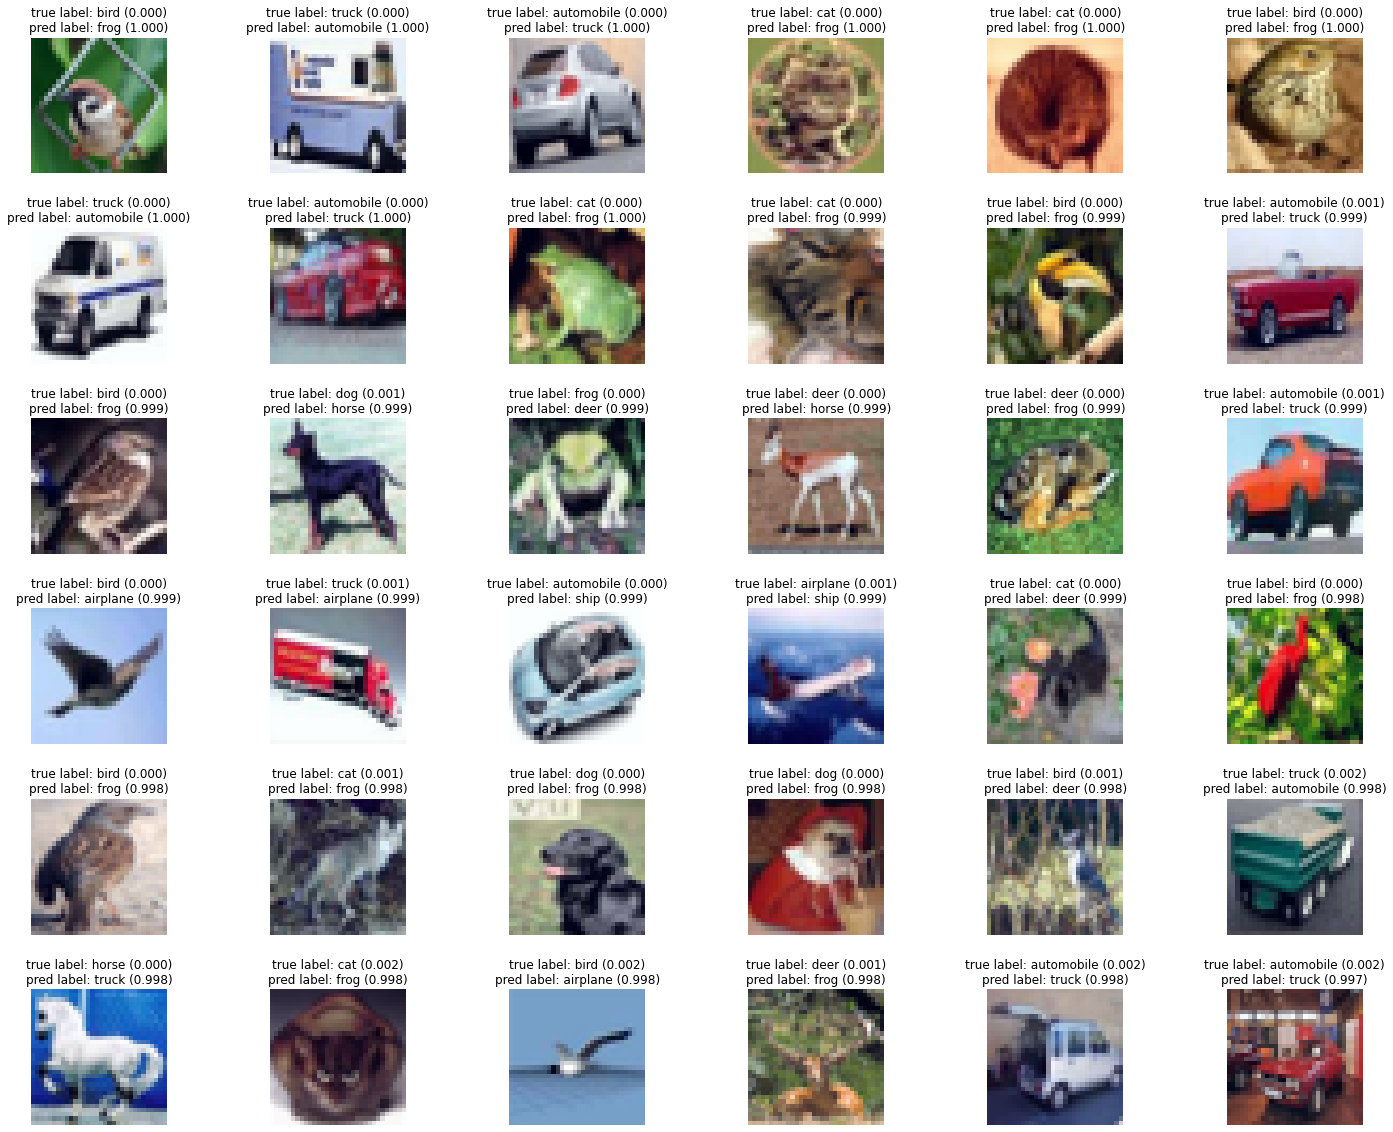
\includegraphics[scale=0.25]{mostincorrectalex.png}
        \caption{Ejemplos de clases con más errores en la clasificación.}
        \label{fig:mosterror2}
\end{figure}

\item Incluya los resultados t-SNE para la capa última capa de la red: analice estos resultados (proximidad, dispersión, agrupación de clústeres) teniendo en cuenta la apariencia de las imágenes de las diferentes clases, sus características típicas y compare los resultados con los resultados t-SNE en el dataset MNIST.

\begin{figure}[H]
        \centering
        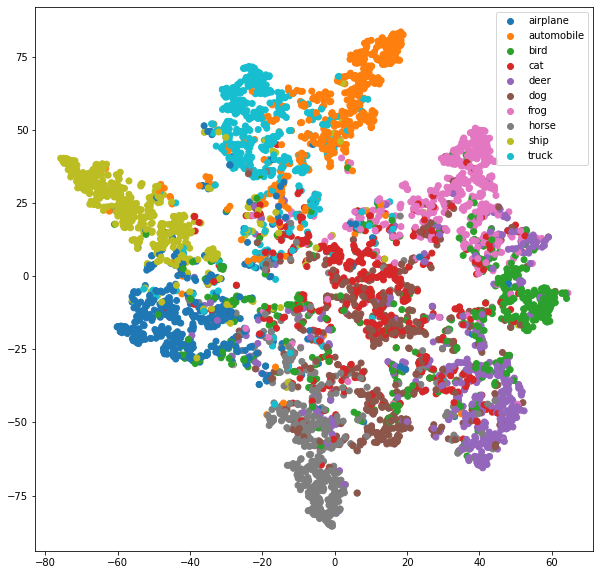
\includegraphics[scale=0.52]{t-snealex.png}
        \caption{Representación final de AlexNet con la proyección t-SNE.}
        \label{fig:sne2}
\end{figure}

En la Figura \ref{fig:sne2} vemos que no se observan clusters tan diferenciados como en el anterior dataset con la otra red, si bien se pueden diferenciar igualmente la mayor parte de las regiones. Comprobamos que los errores han ocurrido en la mayor parte en las clases que hemos mencionado antes, además del caso de los pájaros. Asimismo, vemos que este caso no es tan bueno y que requiere de una mejora. Las maneras de mejorar esto son diversas, entre las cuales se encuentra una mejor optimización de hiperparámetros, en concreto cambiar el \emph{learning rate} o el tamaño de \emph{batch}. También podríamos realizar técnicas de \emph{data augmentation} para aumentar y derivar de los ejemplos que se tienen del dataset, con el fin de enriquecer mucho más al modelo, si bien esto pueda tener un efecto contraproducente en el tiempo de entrenamiento.

\end{itemize}

\section{Transfer Learning}

\begin{itemize}
    \item Precisiones obtenidas para las diferentes alternativas analizadas.
    \begin{table}[H]
    \centering
    \begin{tabular}{l c l l l}
    \multicolumn{1}{c}{}            & \cellcolor[HTML]{E3E7EC}Desde cero & \cellcolor[HTML]{E3E7EC}Pre-entrenamiento + SVM & \cellcolor[HTML]{E3E7EC}Ajuste fino & \cellcolor[HTML]{E3E7EC}Ajuste fino + DA \\ \hline
    \cellcolor[HTML]{E3E7EC}Precisión &  \multicolumn{1}{c}{72.00\%} & \multicolumn{1}{c}{90.50\%}  & \multicolumn{1}{c}{93.50\%} & \multicolumn{1}{c}{95.00\%}\\ 
    \end{tabular}
    \caption{Resultados obtenidos con aprendizaje por transferencia con el dataset Alien.}
    \label{table:restrans}
    \end{table}
    \item Compare las representaciones t-SNE de las diferentes alternativas: entrenamiento desde cero, pre-entrenamiento + SVM, ajuste fino (sin data augmentation) y ajuste fino (con data augmentation) A partir de las diferentes representaciones obtenidas, en las cuatro alternativas analizadas., comente sus diferencias en cuanto a la capacidad de separar linealmente ambas clases, y el nivel de muestras clasificadas erróneamente dada esta separación lineal.
    
    En la Figura \ref{fig:tsne2} se muestran las proyecciones t-SNE obtenidas para cada uno de los métodos, con un hiperplano que separa ambas clases.
    
    Realizamos las siguientes observaciones para cada uno de los métodos:
    
    \begin{itemize}
        \item Desde cero: las clases no están muy separadas a diferencia de otros métodos.
        \item Pre-entrenamiento + SVM: vemos que hay una diferencia mucho más notable de la separación de clases, aún con varios errores.
        \item Ajuste fino: parece que mejora bastante más la clasificación.
        \item Ajuste fino: comprobamos que el efecto de data augmentation es considerablemente bueno para estos datos y esta red. Existen pocos errores y la separabilidad es clara.
    \end{itemize}
    
    Parece que data augmentation es una buena técnica de mejora de los resultados, si bien hay que controlar un poco la cantidad de datos nuevos que generamos y perfeccionar las técnicas utilizadas de cara a otros datasets. No sabemos si esto es generalizable para cualquier dataset, pero desde luego que parece una técnica prometedora para la mejora del rendimiento de estas redes en clasificación de imágenes.
    
    \begin{figure}[H]
        \centering
        \subfigure[Desde cero]{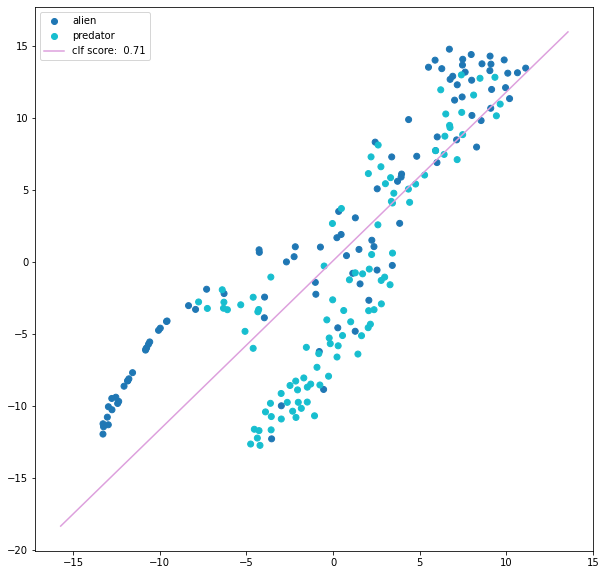
\includegraphics[width=0.4\textwidth]{alien1.png}}   
        \subfigure[Pre-entrenamiento + SVM]{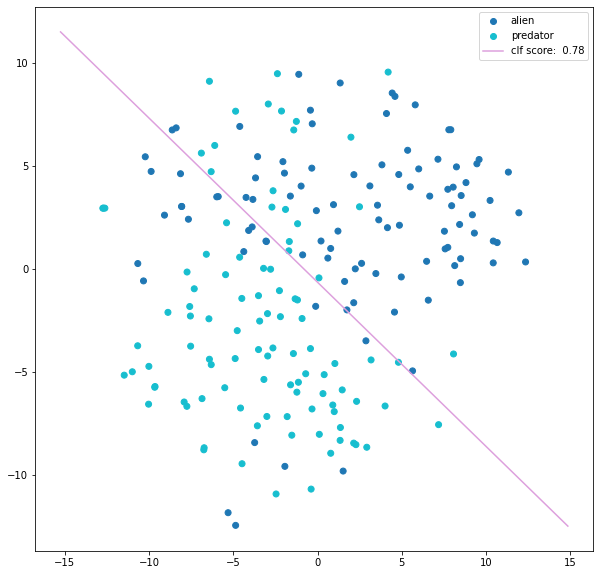
\includegraphics[width=0.4\textwidth]{alien2.png}}
        \subfigure[Ajuste fino]{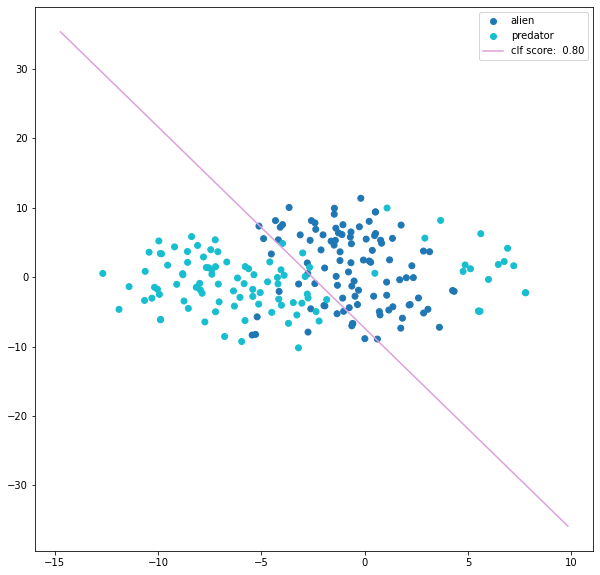
\includegraphics[width=0.4\textwidth]{alien3.png}}
        \subfigure[Ajuste fino + Data Augmentation]{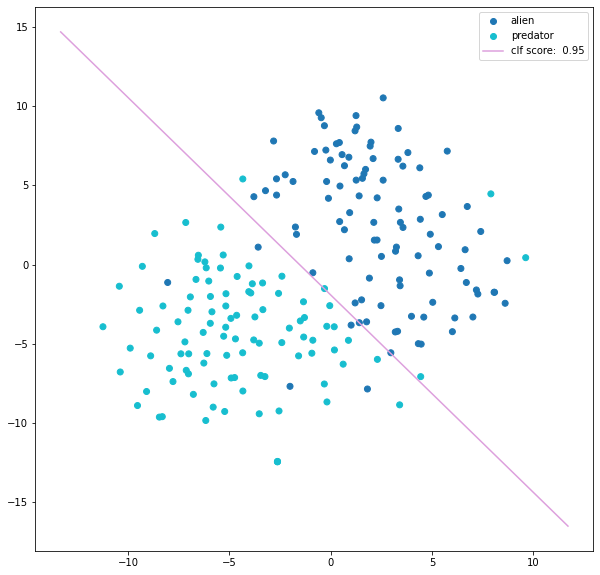
\includegraphics[width=0.4\textwidth]{alien4.png}}
        \caption{Representaciones t-SNE para cada uno de los métodos probados.}
        \label{fig:tsne2}
    \end{figure}
    
\end{itemize}


    
\end{document}